\documentclass[12pt,a4paper]{article}
\usepackage{amsmath,amsthm,amsfonts,amssymb,amscd}
\usepackage{times}     
\usepackage{bookmark}         
\usepackage{graphicx}           
\usepackage{float}              
\usepackage{booktabs}           
\usepackage{xcolor}             
\usepackage{geometry}           
\usepackage{fullpage}           
\usepackage{comment}                     
\usepackage{listings}           
\usepackage{lastpage}           
\usepackage{fancyhdr}           
\usepackage{hyperref}           
\usepackage[small,bf]{caption}  
\usepackage{multicol}
\usepackage{tikz}               
\usepackage{circuitikz}         
\usepackage{verbatim}          
\usepackage{cite}               
\usepackage[us]{datetime} 
\usepackage{blindtext}
\usepackage[utf8]{vietnam}
\usepackage{array}
\usepackage{makecell}
\usepackage{tabularx}
\usepackage{titlesec}
\usepackage{enumitem}

\setlength\parindent{0pt}

%%%%%%%%%%%%%%%%%%%%%%%%%%%%%%%%%%%%%%%%%%%%%%%%%%%%%%%%%%%%%%
\titleformat{\section}
{\color{UM_DarkBlue}\normalfont\large\bfseries}
{\color{UM_DarkBlue}\thesection}{1em}{}

%%%%%%%%%%%%%%%%%%%%%%%%%%%%%%%%%%%%%%%%%%%%%%%%%%%%%%%%%%%%%%
\hypersetup{
    draft=false,
    final=true,
    colorlinks=true,
    citecolor=UM_DarkBlue,
    anchorcolor=yellow,
    linkcolor=UM_DarkBlue,
    urlcolor=UM_DarkBlue,
    filecolor=green,      
    pdfpagemode=FullScreen,
    bookmarksopen=false
    }
    
%%%%%%%%%%%%%%%%%%%%%%%%%%%%%%%%%%%%%%%%%%%%%%%%%%%%%%%%%%%%%%
\lstdefinestyle{Fortran}{
basicstyle=\scriptsize,        % the size of the fonts that are used for the code
  breakatwhitespace=false,         % sets if automatic breaks should only happen at whitespace
  breaklines=false,                 % sets automatic line breaking
  captionpos=b,                    % sets the caption-position to bottom
  commentstyle=\color{mygreen},    % comment style
  extendedchars=true,              % lets you use non-ASCII characters; for 8-bits encodings only, does not work with UTF-8
  keepspaces=true,                 % keeps spaces in text, useful for keeping indentation of code (possibly needs columns=flexible)
  keywordstyle=\color{blue},       % keyword style
  language=[95]Fortran,                 % the language of the code
  numbers=left,                    % where to put the line-numbers; possible values are (none, left, right)
  numbersep=5pt,                   % how far the line-numbers are from the code
  numberstyle=\tiny\color{mygray}, % the style that is used for the line-numbers
  rulecolor=\color{black},         % if not set, the frame-color may be changed on line-breaks within not-black text (e.g. comments (green here))
  showspaces=false,                % show spaces everywhere adding particular underscores; it overrides 'showstringspaces'
  showstringspaces=false,          % underline spaces within strings only
  showtabs=false,                  % show tabs within strings adding particular underscores
  stepnumber=1,                    % the step between two line-numbers. If it's 1, each line will be numbered
  stringstyle=\color{mymauve},     % string literal style
  tabsize=4,                       % sets default tabsize to 2 spaces
  title=\lstname                   % show the filename of files
}

%%%%%%%%%%%%%%%%%%%%%%%%%%%%%%%%%%%%%%%%%%%%%%%%%%%%%%%%%%%%%%%
\definecolor{UM_Brown}{HTML}{3D190D}
\definecolor{UM_DarkBlue}{HTML}{2264B0}
\definecolor{UM_LightBlue}{HTML}{1CA9E1}
\definecolor{UM_Orange}{HTML}{fEB415}




%\newcommand{\tu}[1]{\textup{#1}}
\newcommand{\tu}[1]{\mathrm{#1}}







\newcommand{\ones}{\mathbf 1}
\newcommand{\reals}{{\mbox{\bf R}}}
\newcommand{\integers}{{\mbox{\bf Z}}}
\newcommand{\symm}{{\mbox{\bf S}}}  % symmetric matrices

\newcommand{\nullspace}{{\mathcal N}}
\newcommand{\range}{{\mathcal R}}
\newcommand{\Rank}{\mathop{\bf Rank}}
\newcommand{\Tr}{\mathop{\bf Tr}}
\newcommand{\diag}{\mathop{\bf diag}}
\newcommand{\card}{\mathop{\bf card}}
\newcommand{\rank}{\mathop{\bf rank}}
\newcommand{\conv}{\mathop{\bf conv}}
\newcommand{\prox}{\mathbf{prox}}

\newcommand{\Expect}{\mathop{\bf E{}}}
\newcommand{\Prob}{\mathop{\bf Prob}}
\newcommand{\Co}{{\mathop {\bf Co}}} % convex hull
\newcommand{\dist}{\mathop{\bf dist{}}}
\newcommand{\argmin}{\mathop{\rm argmin}}
\newcommand{\argmax}{\mathop{\rm argmax}}
\newcommand{\epi}{\mathop{\bf epi}} % epigraph
\newcommand{\Vol}{\mathop{\bf vol}}
\newcommand{\dom}{\mathop{\bf dom}} % domain
\newcommand{\intr}{\mathop{\bf int}}
\newcommand{\sign}{\mathop{\bf sign}}

\newcommand{\cf}{{\it cf.}}
\newcommand{\eg}{{\it e.g.}}
\newcommand{\ie}{{\it i.e.}}
\newcommand{\etc}{{\it etc.}}

\graphicspath{{Figs/}}

\begin{document}

\textcolor{UM_Brown}{
\begin{minipage}{0.1\textwidth}
    \begin{flushleft}
        \includegraphics[height=3.5cm]{logo.eps}
    \end{flushleft}
\end{minipage}
\begin{minipage}{0.8\textwidth}
    \begin{center}
        \textbf{\Large Nhập môn mạng máy tính}\\
        \vspace{5pt}
        Assignment 4 \\
        \vspace{20pt}
        \textit{Group 9 - FOBE} \\
        \vspace{5pt}
        \longdate\today
    \end{center}
\end{minipage}
\vspace{10pt}
\hrule
}

\section*{Problem 1: Distributed Hash Table}
\subsection*{1.\;Định nghĩa bảng Hash}
Bảng băm phân tán (Distributed Hash Table - DHT) là một lớp các hệ thống phân tán không tập trung, cung cấp dịch vụ tra cứu tương tự như một bảng băm: các cặp (khóa, giá trị) được lưu trữ trong DHT, và bất kỳ nút mạng tham gia nào cũng có thể lấy được giá trị liên kết với một khóa cho trước một cách hiệu quả. Nhiệm vụ lưu trữ ánh xạ từ khóa tới giá trị được phân tán giữa các nút, bằng cách đó sẽ giảm bớt lỗi nếu có thay đổi trong một tập hợp các nút tham gia. Điều này cho phép sử dụng DHT cho một số lượng cực lớn các nút mạng và xử lý việc vào, ra, và lỗi các nút mạng một cách liên tục.

\begin{figure}[h]
    \centering
    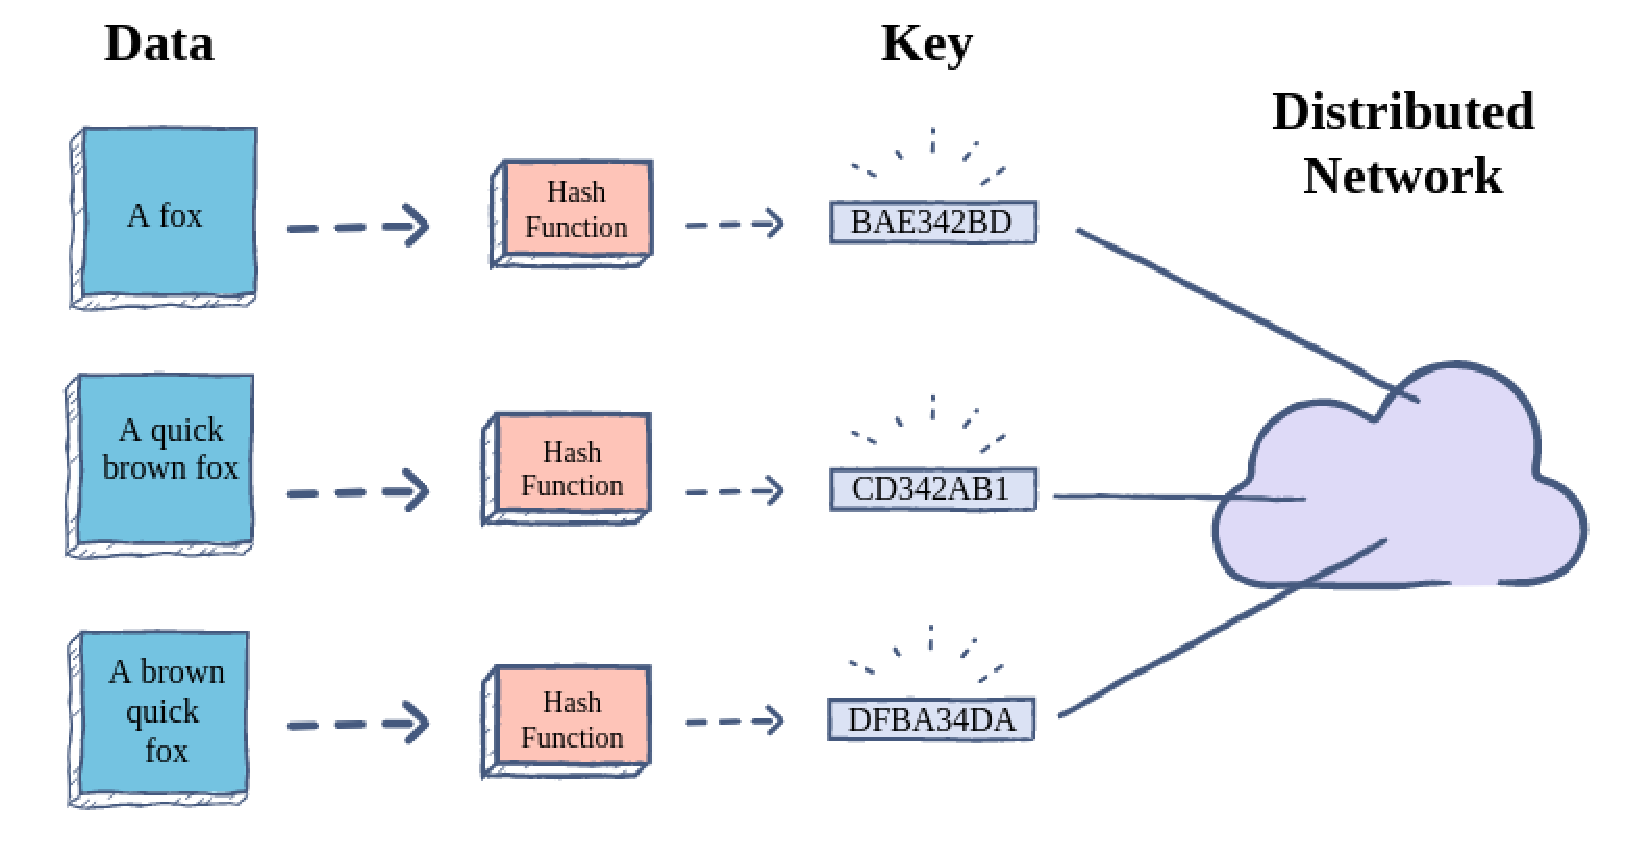
\includegraphics[scale=0.5]{dht.eps}
\end{figure}

\subsection*{2.\; Ứng dụng của DHT}
DHT tạo nên cơ sở hạ tầng cho việc xây dựng các dịch vụ phức tạp hơn, chẳng hạn như các hệ thống file phân tán, chia sẻ file trong mạng đồng đẳng, hệ thống phân phối nội dung (content distribution), web cache có tính hợp tác, multicast, anycast, dịch vụ tên miền và instant messaging. Các mạng phân tán nổi tiếng sử dụng DHT bao gồm máy theo dõi phân tán của BitTorrent, mạng eDonkey, mạng bot Storm, YaCy, và Coral Content Distribution Network.

\newpage
\section*{Problem 2: Checksum}
\subsection*{1.\;Checksum dùng để làm gì ?}
Giá trị tổng kiểm (Checksum) là một giá trị tính toán dùng để gắn vào một gói dữ liệu, dùng để dò tìm các lỗi trong các segment đã được truyền. Tính toán checksum của segment đã nhận, nếu không bằng với giá trị trong trường checksum bên gửi đặt thì đã có lỗi xảy ra.

\begin{figure}[h]
    \centering
    \includegraphics[scale=0.2]{checksum.eps}
    \caption{Input to checksum}
\end{figure}


\subsection*{2.\;Ví dụ tính checksum 16-bit}
Giả sử ta có 3 chuỗi 16-bit như sau:
\begin{flalign*} 
    \hspace{1.5cm} 0110 \; 0110 \; 0110 \; 0000 && \\
    \hspace{1.5cm} 0101 \; 0101 \; 0101 \; 0101 && \\
    \hspace{1.5cm} 1000 \; 1111 \; 0000 \; 1100 && \\
\end{flalign*}
Tổng của 2 chuỗi 16-bit đầu tiên là:
\begin{flalign*} 
    \hspace{1.5cm} 0110 \; 0110 \; 0110 \; 0000 && \\
    \hspace{1.5cm} \underline{0101 \; 0101 \; 0101 \; 0101} && \\
    \hspace{1.5cm} 1011 \; 1011 \; 1011 \; 0101 && \\
\end{flalign*}
Cộng chuỗi 16-bit thứ 3 vào tổng vừa tính được:
\begin{flalign*} 
    \hspace{1.5cm} 0101 \; 0101 \; 0101 \; 0101 && \\
    \hspace{1.5cm} \underline{1000 \; 1111 \; 0000 \; 1100} && \\
    \hspace{1.5cm} 0100 \; 1010 \; 1100 \; 0010 && \\
\end{flalign*}
Lưu ý rằng trong phép cộng cuối cùng có xảy ra overflow và đã được xử lí. \\
\begin{flalign*} 
    \hspace{1.5cm} Checksum = 0101 \; 0101 \; 0101 \; 0101 && \\
\end{flalign*}

\section*{Problem 3: Rdt}
\subsection*{1.\;Vì sao phải dùng các nguyên lí truyền đáng tin cậy ?}
\begin{itemize}
    \item Đảm bảo dữ liệu được gửi đến thành công;
    \item Dữ liệu được gửi đến đúng thứ tự và không trùng lặp;
    \item Hạn chế mất mát dữ liệu;
    \item Mở rộng tốc độ truyền tải
\end{itemize}
\subsection*{2.\;So sánh các phiên bản RDT}

\begin{description}[font=$\bullet$~\normalfont\scshape\color{red!50!black}]
    \item [Rdt 1.0] Đường truyền lí tưởng
\end{description}
Giả định rằng kênh truyền bên dưới tuyệt đối không xảy ra lỗi bit và mất gói tin. \\
\begin{figure}[h]
    \centering
    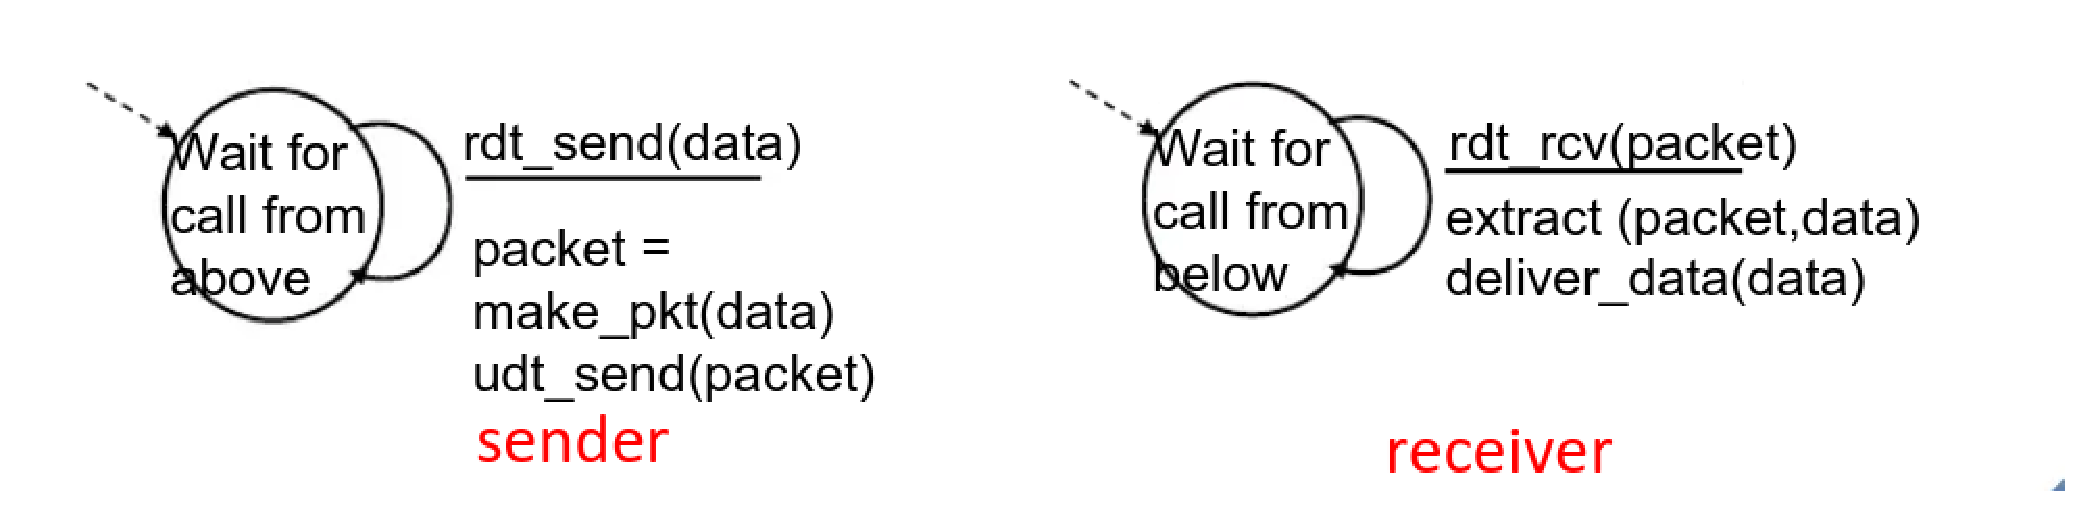
\includegraphics[scale=0.45]{rdt1.eps}
    \caption{Bên nhận và bên gửi Rdt 1.0}
\end{figure}

\begin{description}[font=$\bullet$~\normalfont\scshape\color{red!50!black}]
    \item [Rdt 2.0] Kênh truyền có thể xảy ra lỗi bit
\end{description}
Sử dụng các cơ chế kiểm tra lỗi: \textit{Checksum} \\
Cách khắc phục khi nhận ra lỗi:
\begin{itemize}
    \item Acknowledgement(ACKs): bên nhận báo cho bên gửi đã nhận được dữ liệu
    \item Nagetiveacknowledgement(NAKs): bên nhận báo gói tin bị lỗi
    \item Bên gửi sẽ gửi lại gói tin khi nhận NAK
\end{itemize}
\textbf{So với rdt1.0, rdt2.0 có cơ chế phản hồi ACK, NAK để nhận dạng lỗi}
\begin{figure}[h]
    \centering
    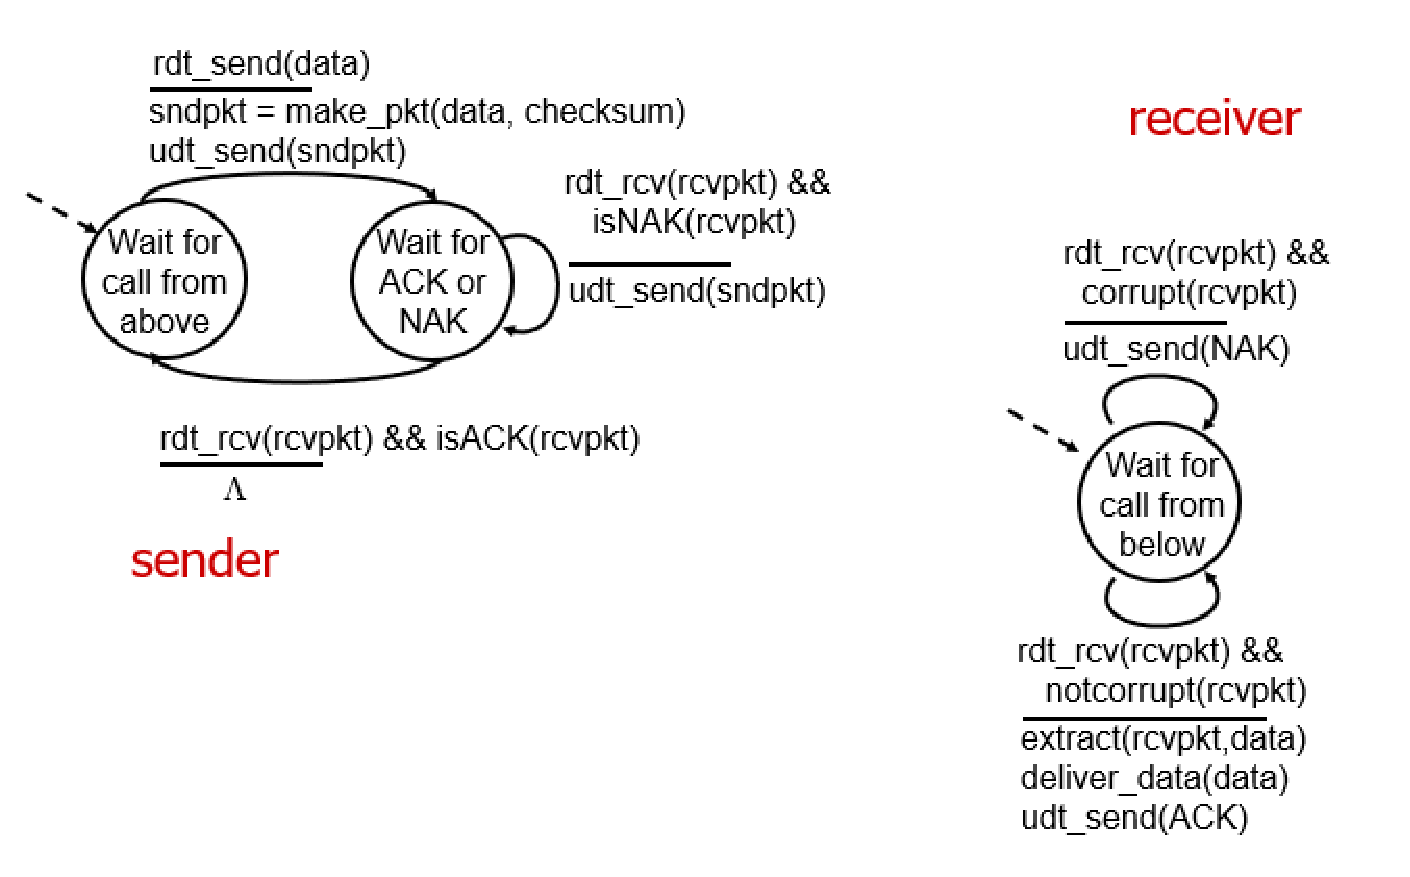
\includegraphics[scale=0.45]{rdt2.eps}
    \caption{FSM bên nhận và bên gửi của Rdt 2.0}
\end{figure}

\begin{description}[font=$\bullet$~\normalfont\scshape\color{red!50!black}]
    \item [Rdt 2.1] Phương thức cải tiến của Rdt 2.0
\end{description}
Rdt 2.0 cung cấp ACK và NAK để giải quyết trường hợp gói tin bị gián đoạn. Tuy nhiên trong
trường hợp chính ACK hoặc NAK bị gián đoạn thì Rdt 2.0 rất có thể sẽ gặp lỗi. Rdt 2.1 giải quyết
vấn đề này bằng Sequence number \\

\begin{description}[font=$\bullet$~\normalfont\scshape\color{red!50!black}]
    \item [Rdt 3.0] Kênh truyền với lỗi và mất mát
\end{description}
Bên gửi đợi một khoảng thời gian hợp lí cho ACK \\
Gửi lại nếu không nhận được ACK không khoảng thời gian này \\
Nếu gói tin (hay ACK) bị trễ (không mất)
\begin{itemize}
    \item Gửi lại có thể trùng, phải đánh số thứ tự
    \item Bên nhận phải xác định thứ tự của gói tin đã ACK
\end{itemize}
Yêu cầu \textbf{đếm thời gian}

\newpage

\section*{Problem 4: FSM của rdt 3.0 bên nhận}
\begin{figure}[h]
    \centering
    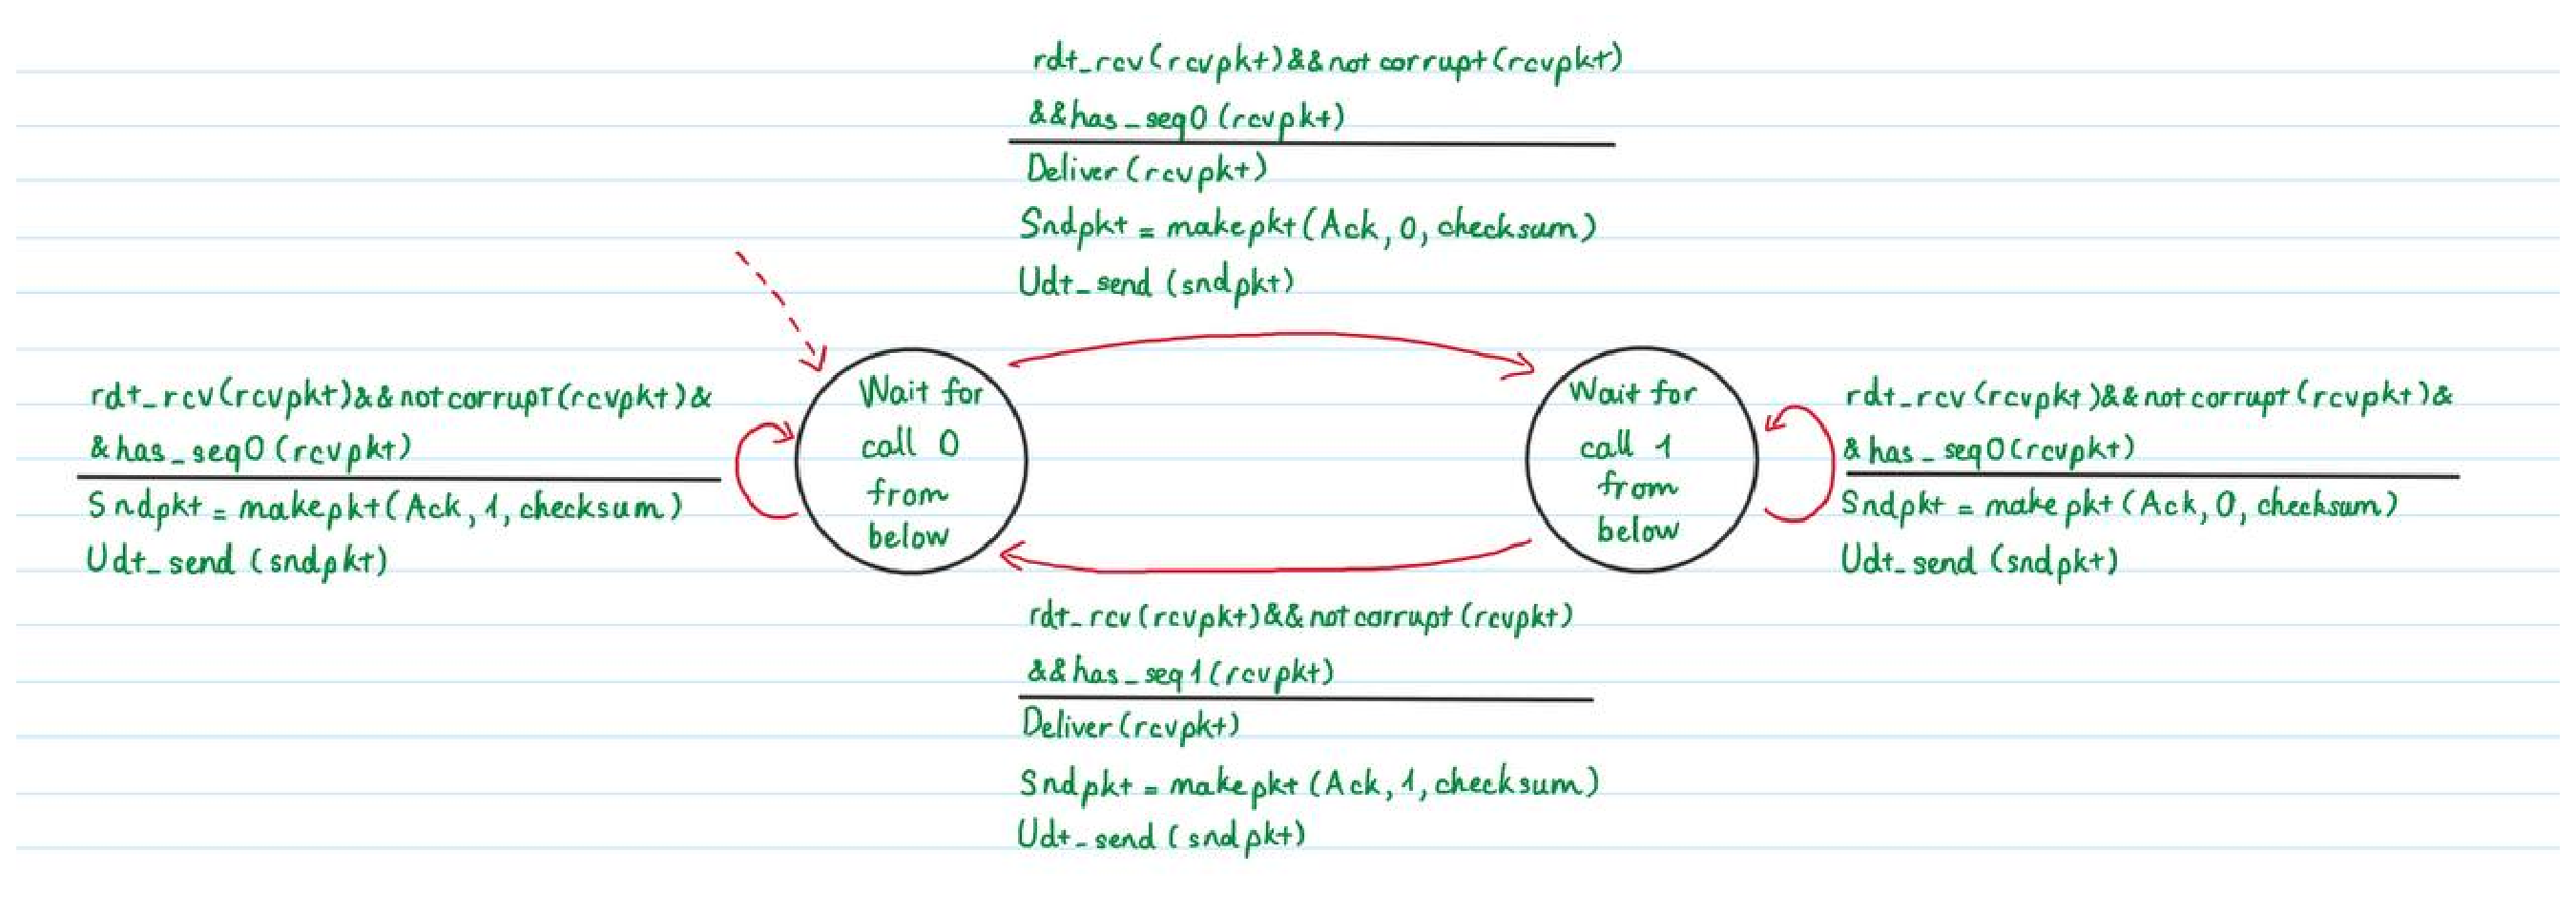
\includegraphics[scale=0.37]{rdt3}
    \caption{Reliable Data Transfer (3.0): Receiver FSM}
\end{figure}

\section*{Contributors and Reference}
\begin{table}[H]
    \caption{Contributors}
    \centering
    \begin{tabular}{c|c}
    \toprule
     \bf{Problem }  & \textbf{Contributors} \\
     \midrule
     1 & Kim Yến \\
     2 & Trâm Anh \\
     3 & Hoàng Tân, Gia Khang \\
     4 & Trâm Anh \\
     \bottomrule
    \end{tabular}
\end{table}

\url{https://en.wikipedia.org/wiki/Distributed_hash_table} \\
\url{https://hazelcast.com/glossary/distributed-hash-table} \\
\url{https://en.wikipedia.org/wiki/Checksum} \\
\url{http://www2.ic.uff.br/~michael/kr1999/3-transport/3_040-principles_rdt.htm}


\end{document} 